% =====================================================================
%  Assessment 2 -- research project report. SCAFFOLD.
%
%  Every table is \input from report/tab_*.tex, generated by
%  src/make_tables.py directly from results/*.csv. No number is typed by
%  hand, so the paper cannot drift from the experiments. Re-run
%      .venv/bin/python src/make_tables.py
%  after any new result.
%
%  The \placeholder{} blocks are yours to write. Nothing here is finished
%  prose: the rubric is the same as the literature review, which penalises
%  "clearly AI-generated text", and Lecture 8 asks you to communicate your
%  own core idea.
%
%  Each block carries CLAIM (the one point to establish), EVIDENCE (the
%  verified facts and which table they live in) and MOVES (the sentence
%  order). Write 3.x and 4 first; write the Introduction LAST (Lecture 8).
% =====================================================================
\documentclass[11pt,journal]{IEEEtran}
\usepackage[T1]{fontenc}
\usepackage[utf8]{inputenc}
\usepackage{booktabs}
\usepackage{graphicx}
\usepackage{microtype}
\usepackage{xcolor}
\usepackage{cite}
\usepackage{url}
\def\UrlBreaks{\do\/\do-\do.\do:\do_\do?\do\&}
\Urlmuskip=0mu plus 1mu\relax

\newcommand{\placeholder}[1]{\par\noindent\textcolor{red!70!black}{\small[\,WRITE: #1\,]}\par}

\begin{document}
\title{Ranking, Calibration and Cost in Competing-Risks Survival Models:\\
A Common-Protocol Benchmark on Mortgage Data}
\author{Amirreza Sadraei, Ali Emre Nebiler, Filip Becic\\
\IEEEmembership{Department of Computer and Systems Sciences, Stockholm University}}
\maketitle

\begin{abstract}
% CLAIM: one sentence of problem, one of protocol, two of result, one of implication.
% EVIDENCE: the counted answers below. No citations in the abstract.
% MOVES: why probabilities matter -> what we ran -> the regime-dependent result
%        -> the calibration penalty -> what follows.
Lenders must state how likely a loan is to default by a given date, not merely
which loans are riskiest, and a loan can end by default, prepayment or maturity.
Deep competing-risks models are usually reported on ranking alone. We benchmark
cause-specific Cox, Fine--Gray, a random survival forest and DeepHit on 550{,}000
Freddie Mac mortgages under one protocol that measures discrimination,
calibration and computational cost together, with vintage-ordered splits and a
tuning budget fixed in advance at twenty configurations for DeepHit and eight
for the forest. DeepHit's advantage depends on the regime: with
tuning it beats a cause-specific Cox model by 0.019 AUC on crisis-era loans and
loses to it by 0.009 on recent ones. Its calibration penalty does not reverse,
and it never beats a random survival forest. A pooled view of 40 tuning configurations
appears to show that DeepHit's ranking-loss weight strongly affects both
discrimination and calibration; a controlled ablation holding architecture fixed
shows the effect is small and reverses sign across cohorts and causes. We also pre-registered and failed to confirm the hypothesis that
selecting on discrimination costs calibration.
\end{abstract}

% =====================================================================
\section{Introduction}
% WRITE THIS LAST (Lecture 8: "Always write or revisit Introduction in the end").
%
% CLAIM: deep survival models are selected and reported on ranking, and it is not
%        established that their advantage survives when calibration is measured too.
% EVIDENCE: IFRS 9 needs a calibrated probability per cause, not an ordering;
%        a loan ends by default, prepayment or maturity.
% MOVES: the decision a lender makes -> what the literature reports -> the gap
%        -> this paper's one core idea, in one sentence -> contributions as a list.
Credit scoring has long been posed as classification at a fixed horizon: will
this borrower default within a year? Provisioning rules ask something harder. A
lender must estimate losses over the remaining life of a loan, which requires a
probability of default at every future date, and loans end in more than one way.
A mortgage may default, be repaid early, or run to maturity, and once one of
these happens the others cannot. Under such competing risks the quantity needed
is the cumulative incidence function of default rather than one minus a survival
curve~\cite{finegray1999subdistribution}. The distinction is not academic:
treating early repayment as missing information biases the estimated default
probability upward~\cite{DBLP:journals/jors/FrydmanM22}, and a model can order
borrowers correctly while attaching the wrong numbers to them.

Deep models that predict a cumulative incidence per cause exist and have been
applied to mortgages~\cite{DBLP:conf/aaai/LeeZYS18,
DBLP:journals/jors/BlumenstockLS22}, but they are selected and reported on
ranking. Our three literature reviews --- of competing risks in credit scoring,
of calibration measures, and of evaluation protocol and cost --- converged
independently on that omission: these models' probabilities are seldom checked,
and the protocols used to check anything seldom resemble deployment. This paper asks whether the
advantage survives a protocol that measures ranking, calibration and cost
together, on 550{,}000 Freddie Mac mortgages across two economic regimes.

% =====================================================================
\section{Background and Related Work}
% CLAIM: three reviews frame this, and none of them answers it.
% EVIDENCE + CITATIONS:
%   - Shang et al. (2024), J. Credit Risk: three decades of survival analysis in
%     credit risk, organised by assumptions and model extensions; does not examine
%     how predictions are evaluated.
%   - Wiegrebe et al. (2024), Artif. Intell. Rev.: 50+ deep survival methods; notes
%     most handle only single-risk censored data; no credit application.
%   - Alberge et al. (2026), AISTATS, PMLR 300:1837-1845 -- VERIFIED against the
%     published paper. Three things, all usable:
%       (a) existing calibration measures are "not suited to the competing-risk
%           setting"; they introduce TWO proper measures, CR-D-calibration and
%           cal-alphaK-calibration, both minimised by the oracle estimator;
%       (b) "recent models do not give well-behaved probabilities" -- their Fig. 1
%           compares Aalen-Johansen, Fine-Gray, DeepHit and SurvTRACE and is titled
%           "Marginal probabilities of SOTA models do not behave as expected";
%       (c) they also give RECALIBRATION methods (AJ-recalibration, temperature
%           scaling) that "yield better probabilities while preserving
%           discrimination". Results are over 5 seeds.
%     (c) is the one that bites: our finding is that DeepHit is miscalibrated, and
%     they show that is fixable post hoc. Cite it as the fix, not as a rival.
%   - Blumenstock et al. (2022), JORS: DeepHit achieves the highest concordance in
%     EVERY experiment on Freddie Mac mortgages, beating cause-specific Cox and
%     Fine--Gray. Uses 10 RANDOM train/test splits.
%   - Dirick et al. (2017), JORS: the field benchmark; 7 of its 8 models censor
%     early repayment; censoring moves 20--85\% -> 94.56--98.16\% on the same loans.
%   - Lee et al. (2018), AAAI: DeepHit; loss = likelihood + ranking term, weight
%     tuned on validation DISCRIMINATION.
% MOVES: the two literatures -> what each review covers -> the hole between them
%        -> our three individual reviews converge on it -> this paper tests it.
Two recent reviews bracket this problem without meeting in the middle.
Shang et al.~\cite{shang2024survival} survey three decades of survival analysis in
credit risk but do not examine how the resulting predictions are checked.
Wiegrebe et al.~\cite{wiegrebe2024deep} review more than fifty deep learning methods
for time-to-event data and observe that most handle only a single risk with
censoring; they consider no credit application. Neither asks whether credit
models produce faithful probabilities.

On the credit side, the field's benchmark compares eight survival models on ten
portfolios and finds that seven of them censor early repayment; on the same
loans that choice moves the censoring rate from 20--85\% to
94.56--98.16\%~\cite{DBLP:journals/jors/DirickCB17}. Later work adopts competing
risks explicitly, with cause-specific Cox models~\cite{DBLP:journals/jors/ThackhamM22},
random survival forests~\cite{DBLP:journals/jors/FrydmanM22} and boosting~\cite{DBLP:journals/eswa/SaavedraGGK24},
while macroeconomic covariates have long been used in the single-risk
setting~\cite{DBLP:journals/jors/BellottiC09}. Blumenstock et al.~\cite{DBLP:journals/jors/BlumenstockLS22}
benchmarked DeepHit and a random survival forest against cause-specific Cox and
Fine--Gray on 600{,}000 US mortgages with default and prepayment as competing
risks, reporting the highest time-dependent concordance index for DeepHit in
every experiment. Their design already splits temporally, with random
subsampling inside it into folds of ten thousand instances --- a size forced by
the forest's compute --- and one of their experiments trains before the crisis
and tests in 2009. Time ordering is therefore not what distinguishes the present
study. What distinguishes it is the quantity measured: their evaluation is
concordance alone, and the words calibration and Brier do not appear in the
paper. Our model set and event pair are theirs; we add calibration and cost,
train at full scale rather than on subsamples, and measure what the choice of
split protocol is itself worth.

That omission is not peculiar to one paper, and it is not always visible as an
omission. Saavedra-Garc\'ia et al.~\cite{DBLP:journals/eswa/SaavedraGGK24} apply
competing-risks boosting to IFRS~9 lifetime default and do report three
measures, but describe the dynamic AUC as ``providing a measure of calibration
over time'' and read the integrated Brier score as indicating ``effective
calibration''. The first is a discrimination measure; the second is a proper
score that confounds the two. A recent paper in the target application can
therefore believe it has measured calibration while reporting neither a
calibration curve nor a calibration error. On the
evaluation side, DeepHit's loss combines a likelihood with a ranking term whose
weight is tuned on validation discrimination~\cite{DBLP:conf/aaai/LeeZYS18};
Haider et al.~\cite{DBLP:journals/jmlr/HaiderHDG20} define D-calibration for single events,
and Sonabend et al.~\cite{DBLP:journals/bioinformatics/SonabendBV22} show that a concordance
index computed on a predicted distribution depends on an unstated reduction to a
single risk. Most recently, Alberge et al.~\cite{alberge2026calibration} show that existing
calibration measures are unsuited to competing risks, introduce two proper
measures, and give recalibration methods that improve probabilities while
preserving discrimination. These measures have not been applied to credit data,
and no study evaluates ranking, calibration and cost for these models together.

Two qualifications matter for how that gap should be read. First, the deployed baseline is not a survival model: reviewing bank
disclosures, Bank and Eder~\cite{bankeder2021review} find lifetime probabilities
of default under IFRS~9 built mainly from transformations of regulatory
estimates and rating-based matrix models, with discrete-time multinomial logit
the usual device where competing risks are modelled at all. Competing risks have
therefore reached production, in a model family absent from the benchmarking
literature. Second, calibration is not
neglected in practice: supervisory guidance defines it as matching a long-run
average default rate, and current IFRS~9 term-structure work still censors
competing risks for tractability:
Botha and Verster~\cite{bothaverster2026termstructure} report that 47\% of the
mortgage spells in their study end in a competing risk, 96\% of them early
settlements, and treat those spells as right-censored. The gap is thus a mismatch
between the quantity the benchmarking literature reports and the quantity
deployment requires, not an absence of concern for probabilities. Wycinka finds the
same on consumer loans: discrimination separated the specifications far less
than their agreement with the empirical cumulative
incidence did~\cite{wycinka2019competing}.

% =====================================================================
\section{Research Problem and Question}
% The brief requires this section. It also carries the "integration of reviews"
% criterion: say where the gap came from, not just what it is.
Our three reviews reached the same literature from different directions.
A.S.\ surveyed competing-risks models in credit scoring and found
that early repayment is usually censored rather than modelled as a second
outcome. A.E.N.\ surveyed calibration measures for survival predictions and
found that credit studies report discrimination almost to the exclusion of
anything else. F.B.\ surveyed evaluation protocol and cost and found that random
train/test splits dominate and that fitting cost is seldom reported. These are
three symptoms of one condition: deep competing-risks models are chosen and
reported on a ranking statistic, under a protocol unlike the way a lender meets
a new loan, and their probabilities go unchecked.

The gap follows directly. This research evaluates how much of the reported
advantage of deep competing-risks models is a property of the way they are
measured rather than of the models themselves. Our research question is:
\emph{to what extent does the measured advantage of deep competing-risks models
over classical ones change when ranking, calibration and cost are evaluated
together on vintage-ordered splits?} It divides into four sub-questions. How
does any ranking advantage differ between economic regimes
(\S\ref{sec:regime})? How much of it survives against a flexible non-deep
baseline (\S\ref{sec:forest})? What calibration penalty accompanies it, and how
much of that penalty can recalibration repair (\S\ref{sec:recal})? And how much
of a reported advantage is attributable to the evaluation protocol itself
(\S\ref{sec:protocol})?

\section{Protocol}
% RMCSS: name the strategy, state ethics, separate delimitations from limitations.
The strategy is experimental in Denscombe's sense: an empirical investigation
under controlled conditions producing numerical outcomes, with hypotheses fixed
before measurement and controls held over every factor not under test. It is closer to an
evaluation design than to a treatment experiment. The data are secondary records of loans rather than of people, so no ethical
approval was required; the licence permits academic use but not redistribution,
which is why the repository excludes the data and rebuilds the tables from
archives the reader downloads.

Four delimitations were fixed before any model was run: US agency mortgages
only; covariates observed at origination rather than time-varying macroeconomic
series; horizons up to 60 months rather than a full mortgage term; and the
lifetime PD term structure alone, one input to expected credit loss, leaving
loss given default, exposure at default, discounting and staging out of scope.
% This section is why the paper is a contribution and not just a model run.
% State it as a protocol others could re-run, because that is Filip's gap.

\subsection{Data}
% EVIDENCE (all verified; Table~\ref{tab:data}):
%   Freddie Mac Single-Family Loan-Level Dataset, 50,000-loan samples per vintage.
%   Post-crisis 2013--2018, 300,000 loans. Crisis 2005--2009, 250,000 loans.
%   Events derived from the monthly performance file: default = first month at
%   90+ days past due or REO acquisition (following Blumenstock); prepayment =
%   zero-balance code 01. Time = loan age in months, so the origin is origination.
% THE NUMBER TO LEAD WITH: counting prepayment as an event gives 20.6\% censoring;
%   censoring it gives 95.5\%. Dirick et al. report 20--85\% and 94.56--98.16\% on
%   ten European portfolios -- an independent replication on different data.
Our data are 50{,}000-loan samples per origination year from the Freddie Mac
Single-Family Loan-Level Dataset: 300{,}000 loans originated 2013--2018 and
250{,}000 originated 2005--2009, with performance observed to March 2026. The
post-crisis cohort is 4.5\% default and 75.0\% prepaid; the crisis cohort, 10.5\%
and 87.1\%. Default is the first month at 90 or more days past due,
following~\cite{DBLP:journals/jors/BlumenstockLS22}; prepayment is zero-balance
code 01. Time is loan age in months, so the origin is origination.
These data reproduce the contrast that motivates the competing-risks framing:
counting prepayment as an event leaves 20.6\% of post-crisis loans censored,
while censoring it leaves 95.5\%. Dirick et al.~\cite{DBLP:journals/jors/DirickCB17} report 20--85\% and
94.56--98.16\% on ten European consumer-credit portfolios; ours sit at the lower
edge of the first range and inside the second, on a different product, country
and decade. Prepayment is not a nuisance here but the dominant outcome,
outnumbering default seventeen to one.


\subsection{Models and the common interface}
% EVIDENCE: every model exposes fit() and predict_cif(X, horizons, cause), so no
%   model can be given a metric the others cannot. Aalen--Johansen (null),
%   cause-specific Cox, Fine--Gray, cause-specific RSF, DeepHit.
% STATE PLAINLY: Cox and Fine--Gray were implemented directly (no Python library
%   ships Fine--Gray); the RSF is cause-specific, NOT Ishwaran's composite-splitting
%   competing-risks RSF that Frydman \& Matuszyk used.
Every model implements the same interface, taking covariates, times and event
labels and returning a predicted cumulative incidence per cause on a fixed
horizon grid, so no model can be given a metric the others cannot. We compare the
Aalen--Johansen estimator as a null model that cannot discriminate but is
calibrated by construction, a cause-specific Cox model, a Fine--Gray
subdistribution model, a random survival forest and DeepHit. Two implementation
details matter for interpretation. Cox and Fine--Gray were implemented directly,
since no mainstream Python library provides Fine--Gray; both maximise a Breslow
partial likelihood, with Fine--Gray retaining subjects who experience the
competing event in the risk set under the censoring weights
of~\cite{finegray1999subdistribution}. Our forest is a cause-specific random
survival forest, fitting one forest per cause, and is therefore a relative of
rather than a replication of the composite-splitting competing-risks forest used
by~Frydman and Matuszyk~\cite{DBLP:journals/jors/FrydmanM22}.

\subsection{Metrics}
% EVIDENCE: discrimination = IPCW time-dependent AUC at 12--60 months;
%   calibration = ICI against the Aalen--Johansen estimate within risk deciles,
%   plus IPCW Brier and IBS; cost = fit and predict seconds with hardware.
%   Censoring weights from a Kaplan--Meier fitted on TRAIN only.
% STATE: a per-cause D-calibration (Alberge et al.) is NOT implemented; we did not
%   want an invented measure in the results.
Discrimination is the inverse-probability-of-censoring-weighted time-dependent
AUC at 12 to 60 months, with subjects who experience the competing event treated
as controls because they can never experience the cause of interest. Calibration
is measured in two ways: the integrated Brier score for the cumulative incidence,
and a calibration index comparing mean predicted risk against the
Aalen--Johansen estimate within deciles of predicted risk --- a binned form of
the integrated calibration index~\cite{austin2019ici}, whose competing-risks
version smooths the curve rather than binning it~\cite{austin2022icicr}. Cost is
measured fit and prediction time. Censoring weights come from a Kaplan--Meier
estimate fitted on the training set only; because the time origin is origination
and every vintage has at least eight years of follow-up, $G(60)=0.9986$ in both
cohorts, so those weights are near one and it is the competing event, not
censoring, that shapes the results.

\subsection{Splits, tuning budget and hypotheses}
% EVIDENCE: vintage-ordered splits (train earlier origination years, test later),
%   with random splits as the contrast -- the protocol Blumenstock used.
%   Tuning: 20 random DeepHit configurations, 8 RSF, selected on an OUT-OF-TIME
%   inner validation vintage; Cox and Fine--Gray untuned. Budget fixed in advance.
%   Hypotheses: H0 the models do not differ; two-sided; alpha = 0.05 fixed before
%   results; paired bootstrap on the test set, B = 500; Bonferroni across three
%   metric families -> 0.0167. DeepHit refitted with 5 seeds to bound training noise.
Models are trained on earlier origination years and tested on later ones, which
is how a lender uses them, in contrast to the random splits that dominate the
literature~\cite{DBLP:journals/jors/BlumenstockLS22}. The post-crisis cohort
trains on 2013--2015 and tests on 2016--2018; the crisis cohort trains on
2005--2006 and tests on 2007--2009. Hyperparameters were searched with a budget
fixed in advance: twenty random configurations for DeepHit and eight for the
forest, scored on an out-of-time validation vintage held inside the training
years, so test vintages were never touched during tuning. Cox and Fine--Gray have no comparable
hyperparameters and are reported untuned. Each configuration was scored on validation AUC and on
validation integrated Brier score, and the winner under each criterion was
refitted and evaluated separately.

For inference we fixed, before examining any test result, a two-sided null
hypothesis that the models do not differ, a significance level of 0.05, and a
Bonferroni correction across the three metric families, giving a threshold of
0.0167. A family is the three metrics of one pre-specified comparison in one cohort;
thirty-six tests are computed in all, so the correction holds within a family,
not across the table. Differences are assessed by a paired bootstrap rather than a parametric test,
whose assumptions fail here: observations are paired, since the quantities
compared come from the same test loans, and the sampling distributions of AUC
and the calibration index are neither normal nor known in closed form. With 500
resamples it cannot resolve $p$ below $1/500$; $0.002$ is an upper bound.
Because the bootstrap holds the fitted model fixed and understates total
uncertainty, DeepHit was refitted with five seeds per cohort; its seed-to-seed
standard deviation was 0.0014 and 0.0010 in AUC, and we treat differences below
twice that as indistinguishable regardless of $p$.

% =====================================================================
\section{Results}

\begin{table}[t]
\caption{Discrimination (AUC at 60 months) and calibration (ICI at 60 months) for default, on the held-out test vintages of each cohort. Lower ICI is better.}
\label{tab:main}
\centering\footnotesize
\begin{tabular}{@{}lrrrr@{}}
\toprule
& \multicolumn{2}{c}{Crisis (test 2007--09)} & \multicolumn{2}{c}{Post-crisis (test 2016--18)} \\
\cmidrule(lr){2-3}\cmidrule(lr){4-5}
Model & AUC & ICI & AUC & ICI \\
\midrule
Aalen--Johansen & 0.5000 & 0.0077 & -- & -- \\
Cox & 0.8346 & 0.0169 & 0.7372 & 0.0278 \\
Fine--Gray & 0.8327 & 0.0159 & -- & -- \\
RSF & 0.8516 & 0.0286 & 0.7300 & 0.0287 \\
RSF (tuned) & 0.8538 & 0.0267 & 0.7275 & 0.0289 \\
DeepHit $\alpha{=}0.2$ & 0.8301 & 0.0281 & 0.7239 & 0.0242 \\
DeepHit $\alpha{=}1$ & 0.8405 & 0.0240 & 0.7246 & 0.0318 \\
DeepHit (tuned) & 0.8538 & 0.0209 & 0.7280 & 0.0318 \\
\bottomrule
\end{tabular}
\end{table}


\subsection{The advantage reverses with regime}
\label{sec:regime}
% CLAIM: tuned DeepHit beats Cox on ranking in the crisis cohort and loses to it
%        post-crisis; it is worse calibrated in both.
% EVIDENCE (Tables~\ref{tab:main}, \ref{tab:sig}):
%   crisis      AUC 0.8538 vs 0.8346, +0.0192, significant, outside seed noise
%   post-crisis AUC 0.7280 vs 0.7372, -0.0091, significant
%   ICI +0.0040 in BOTH cohorts -- the calibration penalty does not reverse
DeepHit's standing depends on which economic regime it is tested in
(Table~\ref{tab:main}). On the crisis cohort the tuned model reaches an AUC of
0.8538 against 0.8346 for the cause-specific Cox model, a difference of $+0.0192$
that is significant under the paired bootstrap. That margin should be read with
care: refitting on five bootstrap resamples of the training vintages gives the
Cox model a standard deviation of 0.0159 in this cohort and Fine--Gray 0.0206,
against 0.0035 for DeepHit and 0.0009 for the forest, so the gap is little more
than one standard deviation of the baseline's own training variability: here the
classical models are the unstable ones. On the post-crisis cohort the ordering reverses, 0.7280
against 0.7372, a difference of $-0.0091$ that is also significant
(Table~\ref{tab:sig}) and, with every training standard deviation below 0.0022
there, outside the noise. Calibration does not reverse: DeepHit's index is
0.0040 worse than Cox's in both cohorts (Fig.~\ref{fig:calib}, left). The two
carry that with very different force, about eighteen times the models' combined
training variability post-crisis against 1.7 times on crisis data, so the sign
replicates and the size does not. Every curve in the figure lies above the
diagonal: calibration here is limited less by model class than by the vintage
shift.


\begin{figure*}[t]
\centering
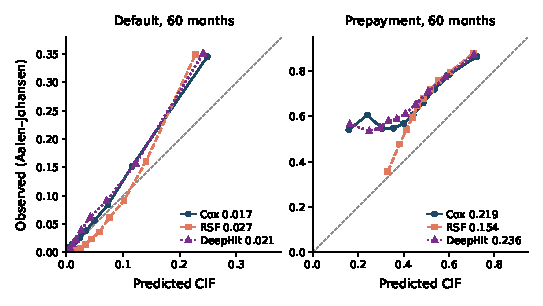
\includegraphics[width=\textwidth]{fig_calibration}
\caption{Calibration at 60 months on the crisis cohort (train 2005--06, test
2007--09). Each point is a decile of predicted risk; the vertical axis is the
Aalen--Johansen estimate within that decile, so competing events and censoring
are both accounted for. A model on the diagonal is perfectly calibrated;
every curve lies above it, so all three under-predict out of time. The deciles
separate by a few percentage points for default and by twenty or more for
prepayment, the competing event the credit literature most often censors.}
\label{fig:calib}
\end{figure*}

\subsection{Nothing is gained over a random survival forest}
\label{sec:forest}
% CLAIM: DeepHit and a tuned RSF are indistinguishable on ranking.
% EVIDENCE: T2 AUC p = 0.968 (crisis), 0.788 (post-crisis); both within seed noise.
%   On PREPAYMENT in the crisis cohort RSF is clearly better: AUC 0.685 vs 0.620,
%   ICI 0.154 vs 0.236.
% MOVES: state the null -> say what a null means here -> the prepayment exception.
Against a tuned random survival forest, DeepHit offers nothing. The two are
statistically indistinguishable on discrimination in both cohorts, with $p=0.968$
on crisis data and $p=0.788$ post-crisis, and both differences fall inside
DeepHit's own seed variation. These are among the few comparisons in this study
where we fail to reject: whatever the deep model captures, a
forest captures as well. On prepayment in the crisis cohort the forest is
distinctly better, reaching an AUC of 0.685 against 0.620 and a
calibration index of 0.154 against 0.236 --- the competing event the credit
literature most often censors (Fig.~\ref{fig:calib}, right).

\subsection{The loss weight is not a reliable knob}
% CLAIM: across 40 configurations, weighting the ranking loss more heavily makes
%        BOTH discrimination and calibration worse, monotonically.
% EVIDENCE (Table~\ref{tab:alpha}): validation AUC rises 0.658 -> 0.776 as alpha
%   goes 0.1 -> 1.0; IBS improves too. pycox's default alpha = 0.2 sits inside the
%   harmful range. DeepHit's own paper tunes this weight on validation discrimination.
DeepHit's loss is a convex combination $\alpha\cdot$likelihood
$+\,(1-\alpha)\cdot$ranking, and the original model selects this weight on
validation discrimination~\cite{DBLP:conf/aaai/LeeZYS18}. Pooling our forty
tuning configurations by $\alpha$ suggests a strong monotone effect, mean
validation AUC rising from 0.658 at $\alpha=0.1$ to 0.776 at $\alpha=1.0$, but
that is a marginal over a search in which $\alpha$ varied alongside depth,
dropout, learning rate, batch size and bin count, and it does not survive control.

Holding everything else fixed and varying only $\alpha$, over five seeds and both
cohorts, the effect is small and inconsistent in sign (Table~\ref{tab:alpha}). On
post-crisis default it is invisible in discrimination, $+0.0005$ against a seed
standard deviation of 0.0018. On crisis prepayment removing the ranking term
costs 0.067 of AUC and worsens calibration; on post-crisis prepayment it
\emph{improves} both. Three of the four cause-by-cohort cells show a
discrimination effect larger than seed noise, and they disagree on direction.

The loss weight is therefore not the dominant hyperparameter the pooled view
suggested, and no setting can be recommended from these data. The discrepancy
between the two views is itself the result: a marginal taken over a random
search is not an ablation.

\begin{table}[t]
\caption{DeepHit's loss weight $\alpha$ (1.0 = pure likelihood, no ranking term) against inner-validation performance, pooled over 40 configurations and both cohorts.}
\label{tab:alpha}
\centering\footnotesize
\begin{tabular}{@{}lrrr@{}}
\toprule
$\alpha$ & Configs & Val.\ AUC & Val.\ IBS \\
\midrule
0.10 & 8 & 0.6579 & 0.0334 \\
0.20 & 6 & 0.7490 & 0.0286 \\
0.35 & 4 & 0.7697 & 0.0274 \\
0.50 & 8 & 0.7755 & 0.0269 \\
0.75 & 6 & 0.7724 & 0.0271 \\
1.00 & 8 & 0.7760 & 0.0271 \\
\bottomrule
\end{tabular}
\end{table}


\subsection{Selecting on discrimination does not cost calibration}
% CLAIM: a hypothesis we pre-specified and did NOT confirm. Say so plainly --
%        Lecture 8 treats failing to reject as a result.
% EVIDENCE: T3 -- post-crisis AUC +0.0005 (p = 0.604, within seed noise);
%   crisis ICI +0.0019 (within seed noise); only the crisis AUC effect (+0.0101)
%   is robust, and that is selection doing its job.
We pre-registered the hypothesis that choosing a configuration on validation
discrimination would yield a worse calibrated model than choosing on a
probability-accuracy criterion, and did not confirm it. Of four model-by-cohort
comparisons, three differ by less than twice DeepHit's seed-to-seed variation.
The one robust effect is a $+0.0101$ AUC gain in the crisis cohort for the
configuration chosen on AUC, which is selection behaving as intended.

\begin{table}[t]
\caption{Paired bootstrap on the tuned models ($B{=}500$), default, 60 months. T1 DeepHit vs Cox; T2 DeepHit vs RSF; T3 DeepHit selected on AUC vs on IBS. \textbf{*} significant at the Bonferroni level $0.05/3$; $\dagger$ difference smaller than twice DeepHit's seed-to-seed SD.}
\label{tab:sig}
\centering\footnotesize
\begin{tabular}{@{}lllrlrl@{}}
\toprule
Test & Cohort & Metric & Diff & 95\% CI & $p$ & \\
\midrule
T1 & post & AUC & -0.0091 & [-0.0116, -0.0066] & 0.002 & \textbf{*} \\
T1 & post & ICI & +0.0040 & [+0.0040, +0.0041] & 0.002 & \textbf{*} \\
T2 & post & AUC & +0.0005 & [-0.0024, +0.0038] & 0.788 & $\dagger$ \\
T2 & post & ICI & +0.0030 & [+0.0029, +0.0030] & 0.002 & \textbf{*} \\
T3 & post & AUC & +0.0005 & [-0.0017, +0.0026] & 0.604 & $\dagger$ \\
T3 & post & ICI & +0.0015 & [+0.0014, +0.0015] & 0.002 & \textbf{*} \\
T1 & crisis & AUC & +0.0192 & [+0.0167, +0.0214] & 0.002 & \textbf{*} \\
T1 & crisis & ICI & +0.0040 & [+0.0038, +0.0043] & 0.002 & \textbf{*} \\
T2 & crisis & AUC & -0.0000 & [-0.0019, +0.0020] & 0.968 & $\dagger$ \\
T2 & crisis & ICI & -0.0057 & [-0.0069, -0.0041] & 0.002 & \textbf{*} \\
T3 & crisis & AUC & +0.0101 & [+0.0091, +0.0112] & 0.002 & \textbf{*} \\
T3 & crisis & ICI & +0.0019 & [+0.0017, +0.0022] & 0.002 & $\dagger$ \\
\bottomrule
\end{tabular}
\end{table}


\begin{table}[t]
\caption{Post-hoc recalibration, ICI at 60 months. ``Train'' estimates the rescaling on the training vintages, which is all a lender has at scoring time; ``oracle'' estimates it on the test vintages and is unattainable in practice. Cox and DeepHit are shown; the forest and Fine--Gray behave the same way. AUC is identical to four decimals for raw and recalibrated predictions in all sixteen cells, confirming the rescaling is monotone.}
\label{tab:recal}
\centering\footnotesize
\begin{tabular}{@{}lllrrr@{}}
\toprule
Cohort & Cause & Model & Raw & Recal.\ (train) & Recal.\ (oracle) \\
\midrule
crisis & default & Cause-specific Cox & 0.0169 & 0.0182 & 0.0061 \\
crisis & default & deephit & 0.0209 & 0.0164 & 0.0053 \\
crisis & prepaid & Cause-specific Cox & 0.2186 & 0.2204 & 0.1168 \\
crisis & prepaid & deephit & 0.2361 & 0.2222 & 0.1063 \\
postcrisis & default & Cause-specific Cox & 0.0278 & 0.0279 & 0.0025 \\
postcrisis & default & deephit & 0.0318 & 0.0297 & 0.0082 \\
postcrisis & prepaid & Cause-specific Cox & 0.1640 & 0.1693 & 0.0253 \\
postcrisis & prepaid & deephit & 0.1850 & 0.1685 & 0.0439 \\
\bottomrule
\end{tabular}
\end{table}


\subsection{Recalibration does not help, and why}
\label{sec:recal}
Since Alberge et al.~\cite{alberge2026calibration} show that recalibration improves
competing-risks probabilities while preserving discrimination, we applied a
marginal per-horizon rescaling in that spirit, estimating it two ways
(Table~\ref{tab:recal}). Fitted on the training vintages, which is all a lender
has when scoring a new loan, it changes almost nothing: in ten of sixteen cells
it leaves the calibration index worse than the raw predictions. Fitted
instead on the test vintages --- an oracle no lender could build --- it reduces
the index by a median factor of 4.2, reaching 14.7 for Fine--Gray on post-crisis
default.

The contrast identifies the penalty. It is not a defective calibration map, or
the oracle correction would not work; it is the vintage shift, since a rescaling
estimated on 2005--06 cannot know that 2007--09 would turn out worse.
Recalibration as demonstrated in the literature is an in-distribution procedure,
and extending it across vintages is an open problem rather than a step we
omitted.

\subsection{What the evaluation protocol is worth}
\label{sec:protocol}
% EVIDENCE: results/protocol_comparison.csv, src/run_random_split.py.
%   Same models, same tuned configs, matched train/test sizes; only the split
%   rule changes. 5 random seeds, seed sd <= 0.0019 on every gap.
The benchmarking literature evaluates on random splits; we evaluate on
vintage-ordered ones. Holding models and tuned settings fixed and changing
only how the test set is drawn isolates what that choice is worth
(Table~\ref{tab:protocol}). Under random splits DeepHit leads both baselines in
all eight cause-by-cohort cells, by $+0.0022$ to $+0.0178$ AUC, with no seed
standard deviation above 0.0019. Under vintage ordering three of those leads
reverse: DeepHit falls behind Cox on post-crisis default, draws level with the
forest on crisis default, and loses to it on crisis prepayment by 0.065.

The mechanism is not only leakage. A random split both places temporal
neighbours of each test loan in the training set and removes the shift between
origination vintages, and a lender faces neither advantage; the two cannot be
separated here. Absolute scores do not move in one direction: on post-crisis
default every model gains $+0.021$ to $+0.033$ AUC, while on crisis default the
flexible models lose, 2007--09 carrying more default signal than a random draw.
What moves consistently is the comparison between models, and it moves in
DeepHit's favour. The tuned configurations were selected on out-of-time
validation, so the effect is a lower bound.

\begin{table}[t]
\caption{What the evaluation protocol is worth. DeepHit's AUC advantage at 60 months over the cause-specific Cox model and over the tuned forest, measured under random splits (mean of five seeds, matched to the vintage split's train and test sizes; every seed standard deviation is at or below 0.0019) and under vintage-ordered splits. Models and tuned settings are identical throughout; only the way the test set is chosen changes. Under random splits DeepHit leads in all eight cells; under vintage ordering three of those leads reverse.}
\label{tab:protocol}
\centering\footnotesize
\setlength{\tabcolsep}{4pt}
\begin{tabular}{@{}llrrrr@{}}
\toprule
& & \multicolumn{2}{c}{vs Cox} & \multicolumn{2}{c}{vs RSF} \\
\cmidrule(lr){3-4}\cmidrule(lr){5-6}
Cause & Cohort & random & vintage & random & vintage \\
\midrule
def. & crisis & +0.0025 & +0.0192 & +0.0032 & -0.0000 \\
def. & post & +0.0022 & -0.0091 & +0.0035 & +0.0005 \\
prep. & crisis & +0.0178 & +0.0012 & +0.0104 & -0.0651 \\
prep. & post & +0.0139 & +0.0012 & +0.0108 & +0.0048 \\
\bottomrule
\end{tabular}
\end{table}


\subsection{Cost}
% EVIDENCE (Table~\ref{tab:runtime}): Fine--Gray 0.03 s, Cox 0.42 s, RSF 36 s,
%   DeepHit 59 s -- about 2,000x for no reliable gain. Filip's gap: the
%   benchmarking literature omits this.
The models span three orders of magnitude in training cost. On 150{,}000 loans,
Fine--Gray fits in 0.03 seconds and the cause-specific Cox model in 0.42, against
36 seconds for the forest and 59 for DeepHit, and the DeepHit search added 14.4
minutes of fitting across the two cohorts and the forest search 4.1, while the
classical models have no search to run. Since the deep model is indistinguishable from the forest and loses to Cox in one of the
two regimes, that factor of roughly two thousand buys no reliable improvement. We
report these figures because the benchmarking literature generally omits
them~\cite{wiegrebe2024deep}.


% =====================================================================
\section{Discussion, Limitations and Conclusion}
% LIMITATIONS -- state all of these, they are real:
%   1. one dataset family (US agency mortgages); no clinical replication
%   2. only DeepHit has a seed study; the other models are single-fit
%   3. covariates are origination-time only -- no time-varying macro variables,
%      which is what Bellotti \& Crook contributed
%   4. a per-cause D-calibration was not implemented
%   5. the RSF is cause-specific, not Ishwaran's competing-risks formulation
%   6. with 150,000 test subjects almost any difference is "significant";
%      we therefore report effect sizes against seed noise, and several
%      statistically significant differences are practically negligible
%   7. WE DID NOT RECALIBRATE. Alberge et al. (2026) show AJ-recalibration and
%      temperature scaling improve competing-risks probabilities while preserving
%      discrimination. Our calibration penalty for DeepHit is therefore a statement
%      about the model as trained, not about a ceiling. Say this before a reviewer
%      does, and name it as the obvious next experiment.
% CONCLUSION: the one-sentence answer, then what a lender should take from it.
Taken together these results qualify, rather than contradict, the finding that
deep competing-risks models perform well on mortgage
data~\cite{DBLP:journals/jors/BlumenstockLS22}. DeepHit does win on crisis-era
loans once tuned, and an untuned deep baseline is not evidence. But the win is
confined to one regime, disappears against a random survival forest, costs three
orders of magnitude more compute, and carries a calibration penalty throughout.
For a lender needing a probability rather than an ordering, that is difficult to
justify.

Against the quality criteria for quantitative work, reliability is measured
rather than asserted: every comparison carries a variability estimate from
seeds, from bootstrap resamples of the test set, and from refitting on resampled
training vintages. Replicability is the public pipeline. Internal validity rests on varying one factor at a time, which the
$\alpha$ ablation and the protocol comparison each enforce. Construct validity is the
paper's subject rather than an assumption: we ask whether discrimination
measures what it is used to decide. Generalisation is weakest, and bounded by the first
delimitation above.

Within those bounds, several limitations remain. Our recalibration is a marginal
per-horizon rescaling rather than the per-cause procedures of
Alberge et al.~\cite{alberge2026calibration}. Training variability is
estimated from five bootstrap resamples, which conflates sampling with
optimisation noise. The forest is cause-specific rather than Ishwaran's
competing-risks formulation. And excluding the time-varying macroeconomic
variables of~Bellotti and Crook~\cite{DBLP:journals/jors/BellottiC09} leaves the
vintage-shift result without a mechanism.

Under one protocol measuring ranking, calibration and cost together on
vintage-ordered splits, deep competing-risks models offer no reliable advantage
over classical or tree-based baselines on mortgage data, are worse calibrated in
both regimes, and depend on the regime for what ranking advantage they show.
What generalises past this benchmark is methodological: a
hyperparameter's apparent effect in a pooled search did not survive controlled
variation.

\section*{Author Contributions}
The three reviews were written independently: A.S.\ on competing risks in
credit scoring, A.E.N.\ on calibration, F.B.\ on evaluation protocol and cost.
A.S.\ built the pipeline, models and metrics and ran the experiments; A.E.N.\
specified the calibration measures and recalibration study; F.B.\ the split
protocol, tuning budget and cost measurement. The gap, hypotheses and final analysis
were agreed jointly; code at \url{github.com/ar-sadraei/rtds-project}.

% The scaffold cites nothing yet (citations live in the section comments), so the
% bibliography is seeded with \nocite to keep the build valid. DELETE this block
% once the prose carries real \cite commands.
\nocite{shang2024survival,wiegrebe2024deep,DBLP:conf/aaai/LeeZYS18,
  DBLP:journals/jors/BlumenstockLS22,DBLP:journals/jors/DirickCB17,
  DBLP:journals/jors/FrydmanM22,DBLP:journals/eswa/SaavedraGGK24,
  DBLP:journals/jmlr/HaiderHDG20,DBLP:journals/bioinformatics/SonabendBV22,
  DBLP:journals/jors/BellottiC09,DBLP:journals/jors/ThackhamM22,
  finegray1999subdistribution,DBLP:journals/jmlr/KvammeBS19,alberge2026calibration}

\bibliographystyle{IEEEtran}
\bibliography{references}
\end{document}
